\chapter{Literature Review}
\label{chap:litreview}
\lhead{\emph{Literature Review}}
% \linespread{8}

% \doublespacing

\section{Introduction}



As we stand on the precipice of a future molded by artificial intelligence and machine learning, one domain that is experiencing considerable progress is Optical Character Recognition (OCR). In this dynamic and continuously evolving field, there are many techniques which have emerged among the significant game-changers, two of these are the Tesseract OCR engine and Convolutional Recurrent Neural Networks (CRNNs). Tesseract, initially developed by Hewlett-Packard and later adopted by Google, is a pioneering engine that converts images of text into machine-encoded text, offering utilities across numerous applications. On the other hand, CRNNs, a deep learning-based approach, combine the spatial feature extraction capabilities of Convolutional Neural Networks (CNNs) with the sequential data processing capacity of Recurrent Neural Networks (RNNs). These networks have set new benchmarks in the realm of scene text recognition, overcoming the challenges posed by variations in text sizes, fonts, and orientations. This literature review delves into the intricacies of these advanced tools, shedding light on their principles, applications, strengths, and potential areas for improvement, thereby enriching our understanding of current trends in OCR technology and pointing to the future possibilities.


% In addition to these techniques, the selection of the correct font for each sensor is another critical element that affects the accuracy of the OCR system. Despite its importance, this aspect has been less emphasized in existing literature, thereby forming a crucial area of exploration in this study.

This literature review explores the current state of OCR technologies, with a particular focus on Tesseract and CRNN models. It delves into various image preprocessing techniques, emphasizing the unique method of red and green color masking before conversion to grayscale. Lastly, it investigates the role of font selection in enhancing OCR accuracy, thereby setting the context for the subsequent research.

While this review focuses on the capabilities of Tesseract OCR and Convolutional Recurrent Neural Networks (CRNNs) in the OCR domain, it's important to acknowledge that the OCR landscape is not limited to these technologies. Many other methods play equally significant roles in expanding the OCR frontiers and opening up new avenues for research and application. Long Short-Term Memory Networks (LSTMs), Transformers, attention-based OCR models, rule-based systems, Support Vector Machines (SVMs), Hidden Markov Models (HMMs), K-Nearest Neighbors (KNN), and template matching are some of these diverse methodologies that provide unique perspectives and solutions in the OCR realm. Each of these methods has its distinctive advantages, making them optimal for certain types of tasks, as well as its limitations, requiring continuous research and development for enhancement. However, the scope of this review will mainly revolve around Tesseract and CRNNs, while the mentioned methods provide an essential context for understanding the broader OCR ecosystem.

\newpage

\section{Tesseract OCR}

Optical character recognition (OCR) is the process of converting images of text into machine-readable text. Tesseract is an open-source OCR engine that is widely used for a variety of tasks, including document digitization, machine translation, and data entry.

\vspace{1cm}

\begin{figure}[ht]
    \centering
    
\includegraphics[width=0.6\textwidth]{Figures/tesseract_ocr.jpg}
    \caption[Tesseract OCR]{Tesseract OCR}\cite{liTrOCRTransformerBasedOptical2023}
    \label{fig:Tesseract OCR}
\end{figure}


In this literature review, we will discuss five research papers that have been published on Tesseract OCR. These papers cover a wide range of topics, including the accuracy of Tesseract, the performance of Tesseract on different types of documents, and the use of Tesseract for specific applications. Each study presents unique findings, and together they create a comprehensive overview of the current state and potential trajectory of Tesseract OCR. Through a detailed exploration of these works, we aim not only to comprehend the nuances of Tesseract OCR but also to contribute to the burgeoning discourse around its implications and opportunities in our increasingly digitized world

In the paper Benchmarking Object Detection Algorithms for Optical Character Recognition of Odometer Mileage"
\cite{ahujaDetectingVehicleType}


\newpage
\section{Convolutional Recurrent Neural Networks (CRNNs)}

CRNN, an abbreviation for Convolutional Recurrent Neural Network, is a unique fusion of the advantages of convolutional neural networks (CNN) and recurrent neural networks (RNN), which are different kinds of neural network architectures.

CRNNs are usually applied in the classification and analysis of sequential data like text, speech, and images. Due to their ability to handle variable-length sequential data and recognize long-term dependencies, they are extremely useful for tasks that need to comprehend contextual and temporal information. They have displayed excellence in modeling and processing sequential data across diverse tasks, marking them as an efficient instrument in this domain.

\section{Working of CRNNs}
The functionality of CRNNs is outlined as follows:

\begin{enumerate}
    \item \textbf{Input:} The primary input to a CRNN is a sequence of data, which could be images or audio samples.
    \item \textbf{Convolutional Layers:} The incoming sequence is channeled through convolutional layers, akin to those in CNNs. These layers extract features from the input and are particularly efficient for image-based inputs.
    \item \textbf{Recurrent Layers:} The output from a convolutional layer is then sent through one or more recurrent layers. These layers preserve a hidden state that memorizes information from previous entries in the sequence, making them ideal for sequential data processing.
    \item \textbf{Bridge between Convolutional and Recurrent Layers:} Usually, the output from a convolutional layer is sampled before it is introduced to a recurrent layer. This strategy helps to minimize the network's computational complexity while maintaining the core characteristics of the input.
    \item \textbf{Output:} Finally, the output from the last recurrent layer is processed through a fully connected layer. This final layer produces a prediction for the input sequence, which could be a string of characters, words, or any other output related to the task.
\end{enumerate}

\newpage

\section{Other OCR Methods}

\subsection{Long Short-Term Memory Networks (LSTMs)}

Long Short-Term Memory Networks (LSTMs) are a special kind of recurrent neural network capable of learning long-term dependencies, which makes them highly suitable for OCR tasks. They've been used successfully to decode sequences of characters from images.\cite{breuelHighPerformanceOCRPrinted2013}

Breuel et al. in the paper "High-Performance OCR for Printed English and Fraktur using LSTM Networks" write about a novel application of bidirectional Long Short-Term Memory (LSTM) networks to the problem of machine-printed Latin and Fraktur recognition, without segmentation, language modelling or post-processing.

\begin{figure}[ht]
    \centering
    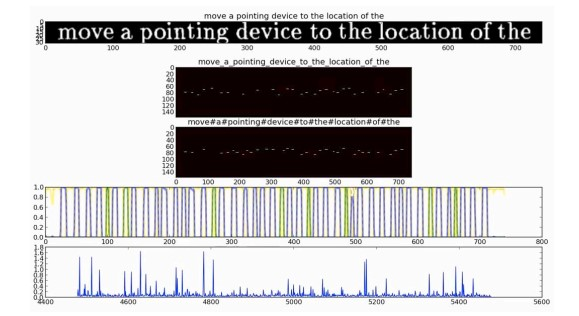
\includegraphics[width=0.8\textwidth]{Figures/LSTM_Breuel.jpg}
    \caption[Bruel's illustration of the training steps of the LSTM recognizer]{Greyscale image with background cleaning}\cite{breuelHighPerformanceOCRPrinted2013}
    \label{fig:Breuel LSTM Paper}
\end{figure}



A preprocessing step for text-line normalisation that uses a dictionary of connected component shapes and associated baseline and x-height information to map the input text lines to a fixed size output image.

A comparison of the LSTM-based system with other OCR systems on printed English and Fraktur texts, showing that LSTM achieves very low error rates and generalizes well to unseen data.

\newpage

\subsection{Transformers}

Originally developed for natural language processing tasks, Transformer models have been adapted for OCR. They treat the OCR problem as a sequence-to-sequence translation task, translating the input image into a sequence of characters.

\begin{figure}[ht]
    \centering
    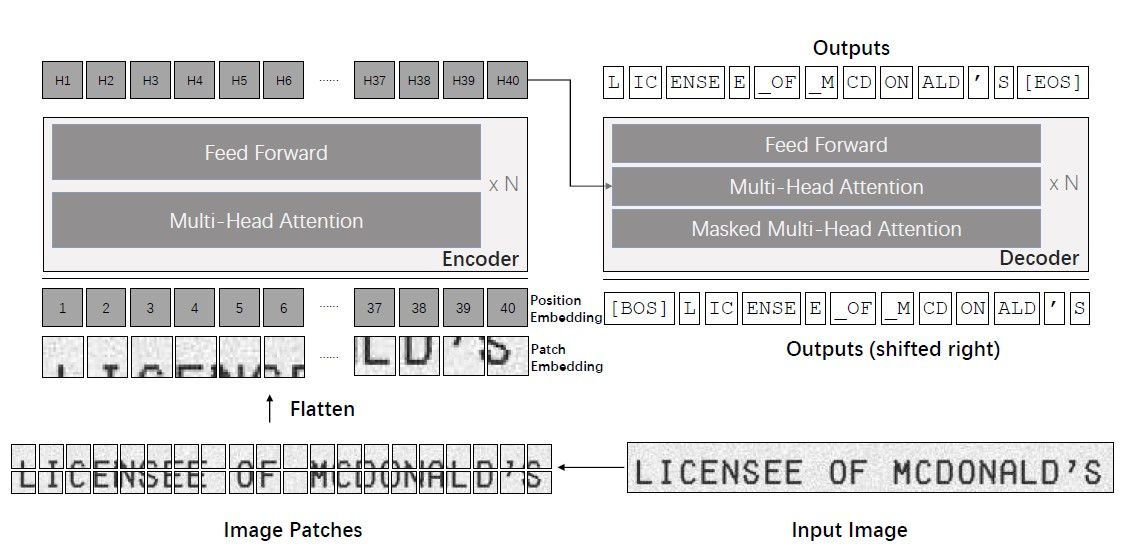
\includegraphics[width=0.6\textwidth]{Figures/Trans_MLi.jpg}
    \caption[Li's Architecture of TrOCR]{Li's Architecture of TrOCR}\cite{liTrOCRTransformerBasedOptical2023}
    \label{fig:Li's Architecture of TrOCR}
\end{figure}

M.Li et al.'s "TrOCR: Transformer-Based Optical Character Recognition with Pre-trained Models" paper proposes an end-to-end text recognition approach with pre-trained image Transformer and text Transformer models, which leverages the Transformer architecture for both image understanding and wordpiece-level text generation. \cite{liTrOCRTransformerBasedOptical2023}

Transformer based OCR models have the advantage of being able to handle long sequences of text, which is useful for OCR tasks. However, they are computationally expensive and require large amounts of training data.

CRNNs are more suitable for this project because they are faster and require less training data and are better at handling spatial information

\newpage

\subsection{Attention-based OCR models}

Attention mechanisms allow models to focus on different parts of the input image while predicting each character in the output sequence, similar to how humans read. This can improve accuracy, especially on more complex images.

Li et al.'s "Attention Based RNN Model for Document Image Quality Assessment" paper proposes a novel method for document image quality assessment (DIQA). The method integrates convolutional neural networks (CNNs) and recurrent neural networks (RNNs) to capture spatial features and attention mechanisms. It also uses reinforcement learning to train a locator network that selects the optimal regions for quality evaluation.

The CNNs are used to extract spatial features from the document images. The RNNs are used to capture the temporal dependencies between the features. The locator network is used to select the optimal regions for quality evaluation. The regions are selected based on the attention mechanism, which identifies the most important regions in the document images. \cite{liAttentionBasedRNN2017}


\begin{figure}[ht]
    \centering
    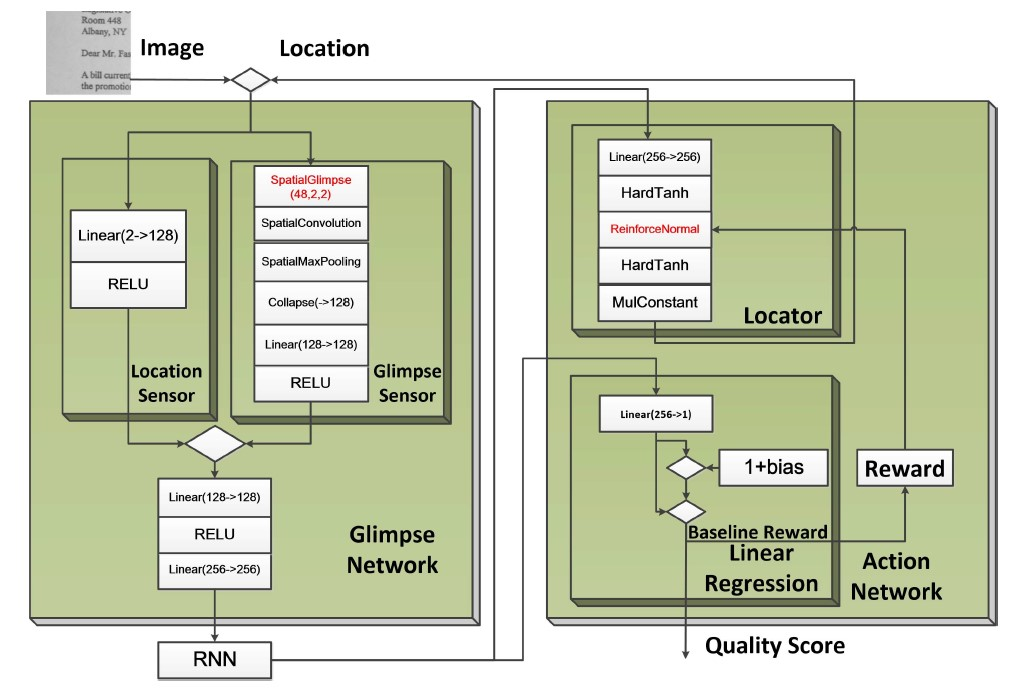
\includegraphics[width=0.6\textwidth]{Figures/AT_Li.jpg}
    \caption[Architecture of Li's proposed network]{Architecture of Li's proposed network}\cite{liAttentionBasedRNN2017}
    \label{fig:Li's Proposed Architecture}
\end{figure}

RNNs are good at handling sequential information but are poor at handling spatial information. CRNN's are more complex and combine the strengths of CNNs and RNNs which is more suitable for the this paper's OCR task.



\newpage

\subsection{Rule-based systems}

These were some of the earliest methods for OCR and use specific rules for identifying characters based on their shape, size, and relative position. They are now less commonly used due to their limitations with complex and diverse inputs.

Doush et al.'s paper "A novel Arabic OCR post-processing using rule-based and word context techniques" developed a rule-based OCR system for Arabic text that uses a combination of horizontal and vertical projections to segment characters and then classifies them based on their shape and relative position. \cite{doushNovelArabicOCR2018}



\begin{figure}[ht]
    \centering
    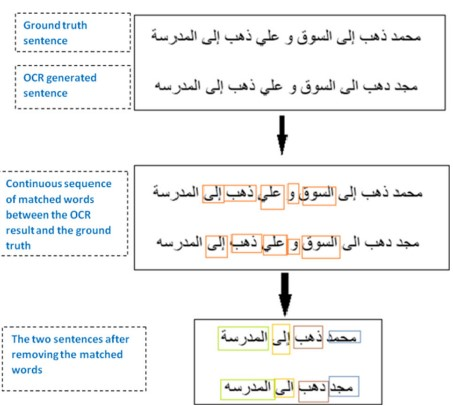
\includegraphics[width=0.6\textwidth]{Figures/RB_Doush.jpg}
    \caption[Example of applying the Rule Based FAHTA Algorithm]{Example of applying the Rule Based FAHTA Algorithm}\cite{doushNovelArabicOCR2018}
    \label{fig:Doush Rule Based OCR Paper}
\end{figure}

The FAHTA algorithm is a novel alignment technique that is used to match the ground truth text with the OCR misrecognized text. The paper also says that the FAHTA algorithm is fast, accurate, and can handle different types of OCR errors, such as over-segmentation, under-segmentation, and merging words. The paper claims that the FAHTA algorithm can be used for other languages as well.


For the purposes of this project, the rule-based system is not suitable because it requires a large number of rules to be defined for each character, which is not feasible for the large range iof digit fonts.


\newpage

\subsection{Support Vector Machines (SVMs)}

Support Vector Machines (SVMs) are used for character recognition in OCR due to their effective high-dimensional mapping and classification abilities. They work best when text is clearly segmented. In the their paper "Development of an Image Processing Techniques for Vehicle Classification Using OCR and SVM", Joshua et al. used SVMs to classify characters in a license plate image and achieved an accuracy of 98.3\% using a local dataset of 10,000 images.\cite{joshuaDevelopmentImageProcessing2023}

\begin{figure}[ht]
    \centering
    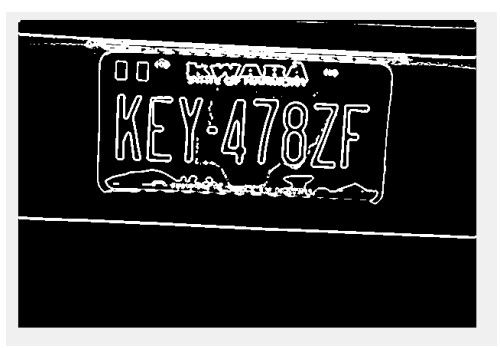
\includegraphics[width=0.8\textwidth]{Figures/SVM_Joshua.jpg}
    \caption[Development of an Image Processing Technique for Vehicle Classification using OCR and SVM]{Greyscale image with background cleaning}\cite{joshuaDevelopmentImageProcessing2023}
    \label{fig:Joshua SVM Paper}
\end{figure}

Joshua et al. describe the steps of their proposed system, which include image preprocessing, feature extraction, OCR, and SVM classification. They also explain how they collected and labeled their dataset of Nigerian vehicle plate numbers.

\newpage

\subsection{Hidden Markov Models (HMMs)}

HMMs have been used in OCR for recognizing sequential data. HMMs are statistical models that assume an underlying process to be a Markov process with hidden states.


In Rashid et al.'s "An evaluation of HMM-based Techniques for the Recognition of Screen Rendered Text" paper, they evaluate Hidden Markov Model (HMM) techniques for optical character recognition (OCR) of low resolution text from screen images and compares them with other OCR systems.

The paper uses two data sets of screen rendered characters and text-lines, and extracts two types of features from them: gray scale raw pixel features and gradient based gray level intensity features.


\begin{figure}[!h]
    \centering
    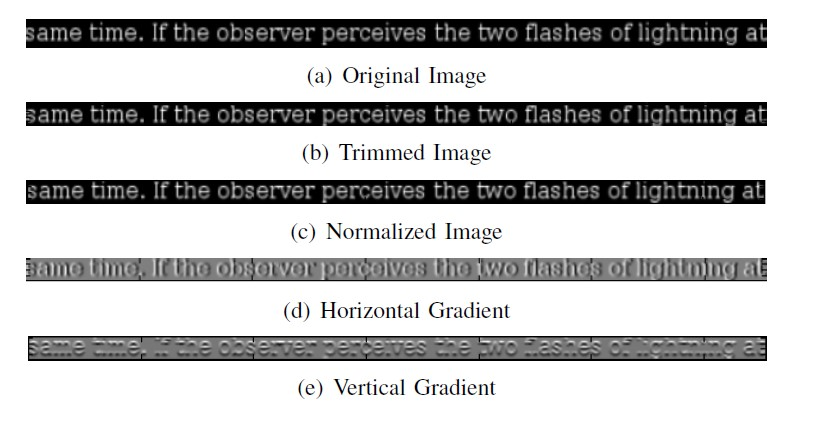
\includegraphics[width=0.8\textwidth]{Figures/HMM_Rashid.jpg}
    \caption[Rashid's Extraction steps from screen rendered text-lines]{Rashid's Extraction steps from screen rendered text-lines}\cite{rashidEvaluationHMMBasedTechniques2011}
    \label{fig:Rashid Feature Extraction Steps}
\end{figure}

The paper reports the character recognition accuracy of the HMM-based methods and other OCR engines on the two data sets. It shows that the HMM-based methods reach the performance of other methods on screen rendered text and achieve above 98\% accuracy.\cite{rashidEvaluationHMMBasedTechniques2011}

HMMs are a good choice for tasks where simplicity and interpretability are important. CRNNs are a good choice for tasks where accuracy is more important, and where the sequences are long or complex.

\newpage

\subsection{K-Nearest Neighbors (KNN)}

KNN is a simple, instance-based learning algorithm used for OCR, particularly for isolated character recognition. Hazra et al. develop an optical character recognition (OCR) system that uses a custom image to train a k-nearest neighbor (KNN) classifier. They claim that their system can recognize handwritten or printed text in any language by changing the training image and labels. \cite{hazraOpticalCharacterRecognition2017}

\begin{figure}[!h]
    \centering
    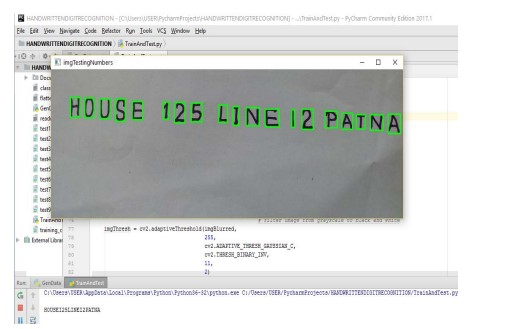
\includegraphics[width=0.8\textwidth]{Figures/KNN_Hazra.jpg}
    \caption[Optical Character Recognition using KNN on Custom
        Image Dataset]{Characters and Digits regocnised}\cite{joshuaDevelopmentImageProcessing2023}
    \label{fig:Hazra OCR KNN Paper}
\end{figure}

Hazra et al. explain the steps of their algorithm, which include image processing, feature extraction, and KNN classification. They also discuss the advantages of KNN over other classification methods, such as ease of interpretation, low computation time, and high predictive power. In this paper the authors started with clear images of known fonts, which is not the case in this project.


\newpage

\subsection{Template Matching}

Template Matching is a technique used to locate small-parts of the bigger image which match a template image. This can be useful in OCR when the set of possible characters is known and limited. In Hossain et al.'s "Optical Character Recognition based on Template Matching" paper, they use template matching to recognize characters in a license plate image.

\begin{figure}[ht]
    \centering
    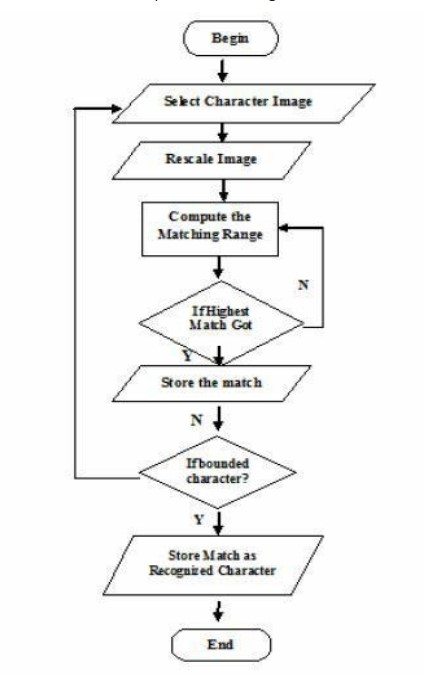
\includegraphics[width=0.4\textwidth]{Figures/TM_Hossain.jpg}
    \caption[Flowchart of Template Matching OCR]{Flowchart of Hossain's TM OCR}\cite{hossainOpticalCharacterRecognition2019}
    \label{fig:Hossain OCR Template Matching Paper}
\end{figure}

Their system prototype was tested on different text images with different fonts and sizes. The accuracy was calculated based on the character recognition accuracy. Their results show that Calibri and Verdana fonts had the highest accuracy, while Cambria and Times New Roman fonts had the lowest accuracy.  The accuracy can be improved by training the system with more fonts and features. \cite{hossainOpticalCharacterRecognition2019}


